
\section{Физические принципы голографии. Голограмма Д. Габора, голограмма Ю.Н. Денисюка.}


\textit{Голография} - это метод точной записи волновый полей с учетом амплитуды и фазы.

\medskip 

Для записи голограммы помимо \textit{предметной волны} от фотографируемого объекта используется еще одна волна, называемая \textit{опорной}. На фотографии записывается результат их интерференции, в результате чего записывается информация о фазе предметной волны (относительно опорной). При освещении голограммы восстанавливающей волной, которая должна быть идентична опорной, получаем обратно предметную волну.



\begin{figure}[h!]
    \centering
    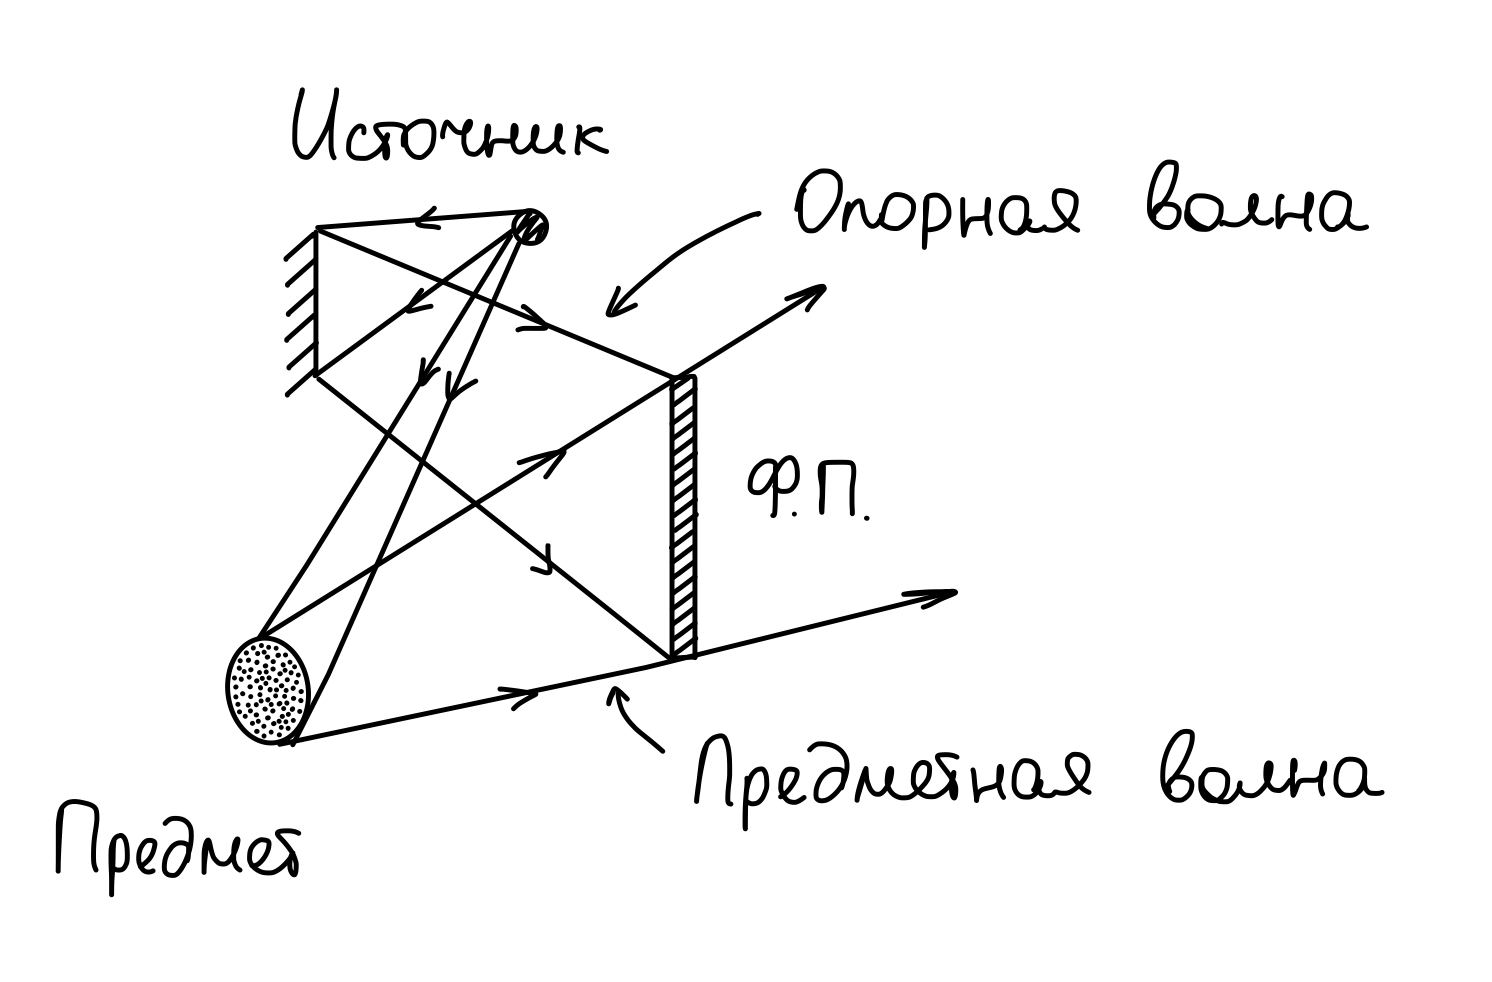
\includegraphics[scale=0.25]{holo1.PNG}
    \caption{Запись голограммы}
    \label{fig:my_label}
\end{figure} 



\begin{figure}[h!]
    \centering
    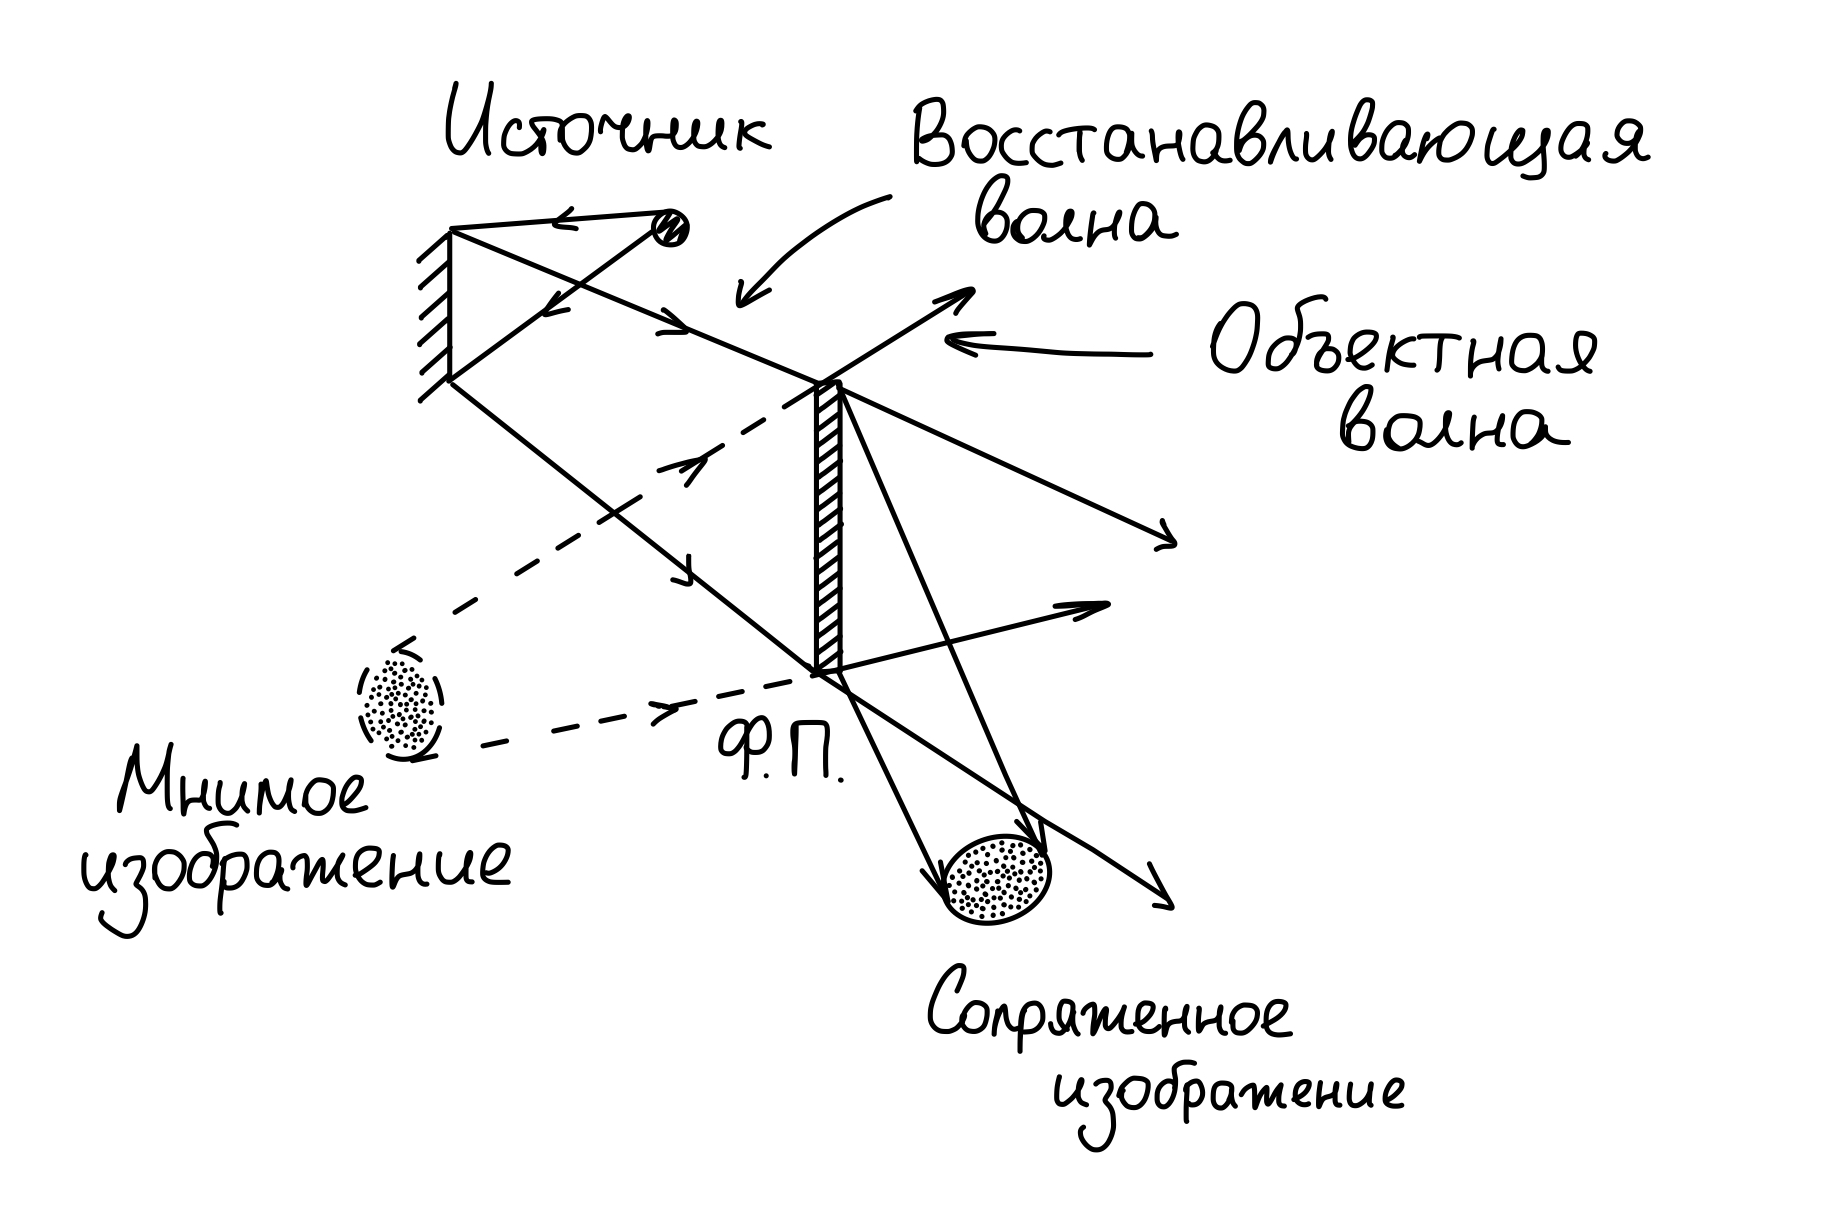
\includegraphics[scale=0.25]{holo2.PNG}
    \caption{Восстановление голограммы}
    \label{fig:my_label}
\end{figure} 
\newpage


\subsection{Голограмма Габора}

Если опорная волна падает по нормали на фотопластинку в том же направлении, что и предметная волна, реализуется \textit{схема Габора}. (Схема описана выше.)
\subsection{Голограмма Денисюка}

Если предметная и опорная волна идут навстречу друг другу, то реализуется \textit{схема Денисюка}. Эта схема используется при записи толстых (объемных) голограмм.

С помощью метода Денисюка получаются трехмерные, объемные голограммы на пластинках с толстослойной эмульсией.

Опорная плоская монохроматическая волна от лазера падает на фотопластинку со стороны стекла. Пройдя через фотопластинку, она освещает голографируемый предмет. Волна, рассеянная предметом, распространяется навстречу опорной волне, интерферируя с ней в толще фотоэмульсии. Интерференционная картина представляет стоячик волны, на который наложен причудливый узор мелких деталей из максимумов и минимумов, так как среди интерферирующих волн только опорная волна является плоской. Проявленная и отфиксированная фотопластинка и будет объемной голограммой Денисюка. Она состоит как бы из нескольких десятков поверхностных голограмм, расположенных в толще эмульсии.

\medskip


Восстановление предметной волны производится расходящимся пучком белого света. Каждый слой выделившегося серебра, действуя подобно двухмерной голограмме, дает слабые мнимое и действительное изображения предмета. При многолучевой интерференции происходит усиление тех волн, длина которых равна длине волны излучения лазера, в тех направлениях, в которых разность фаз между волнами от соседних слоев серебра равна $2\pi$. В результате возникают изображения того же цвета, что и цвет луча лазера. Остальные изображения гасят друг друга при интерференции.

\medskip

Таким образом, голограмма производит монохроматизацию белого света, которым она освещается. Конечно, такая монохромати-зация сравнительно невысокая, из-за незначительного числа отложившихся слоев серебра и связанной с этим небольшой спектральной разрешающей способности голограммы. Кроме того, цвет изображения может существенно отличаться от цвета излучения лазера. Это связано с изменением расстояний между слоями почернения при проявлении, фиксировании и сушке фотопластинки.

\medskip

Метод Денисюка, подобно трехцветной фотографии, позволяет получать изображения предметов в натуральных цветах. Для этого на одной и той же фотопластинке получают голограмму предмета с помощью трех лазеров, излучения которых имеют различные длины волн. Последние подбираются так, чтобы при смешении они наиболее совершенно воспроизводили цвет предмета. Такая голограмма действует как три голограммы, дающие при освещении белым светом совмещенные изображения предмета в трех цветах. При этом цвет изображения кажется глазу таким же, как и цвет самого предмета.
